\documentclass{deck}
\usepackage[T2A]{fontenc}
\usepackage[russian]{babel}
\usepackage{dejavu}
\usepackage{soul}
\usepackage[absolute]{textpos}\TPGrid{16}{16}\ttfamily
\definecolor{background}{HTML}{F0F5F5}\pagecolor{background}
\pagestyle{empty}
\setstretch{1.1}
\sethlcolor{zgreen}
\begin{document}
\setlength{\parindent}{0pt} % indent first line

\setlength{\fboxsep}{2pt}
\newcommand\point[2]{\vbox{\raggedright\small%
  \fcolorbox{zgreen}{white}{\color{zgreen}#1}\newline%
  \footnotesize#2\vspace{16pt}}}
\newcommand\highlight[1]{\colorbox{zgreen}{\color{white}\thinspace{#1}\thinspace}}

\begin{textblock}{7}[0,0](2,13){
  \setstretch{1.0}\color{gray}\footnotesize
  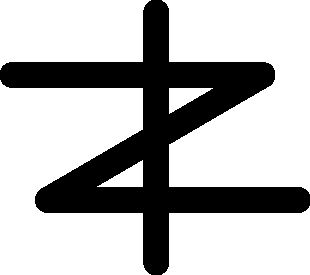
\includegraphics[height=24pt]{../images/zerocracy-logo.pdf}
  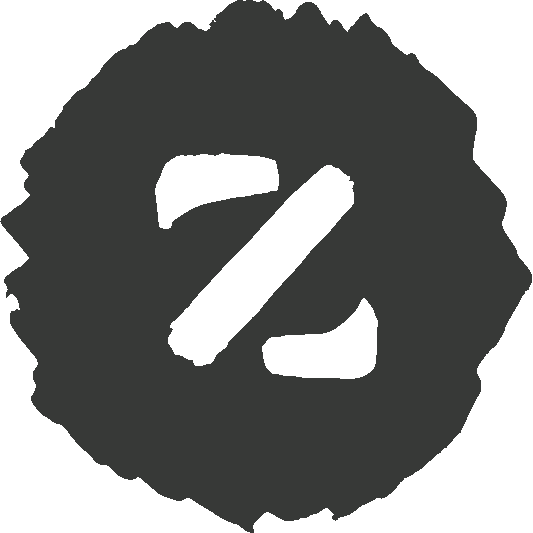
\includegraphics[height=24pt]{../images/logo.pdf}\\
  Это не инвестиционное предложение.,
  Для получения инвестиционных документов, свяжитесь с нами по \href{mailto:cio@zerocracy.com}{емейл}.\\
  555 Bryant Str, Ste 470, Palo Alto, CA 94301, USA\quad+1 (408) 692-4742\\
  \today\quad\zoldversion
}\end{textblock}

\begin{textblock}{7}[1,0](15,13){\begin{flushright}
  \setstretch{1.0}\color{gray}\footnotesize
  О нас пишут:\\
  \href{https://www.rbc.ru/crypto/news/5c0f98a79a79479329c12358}{
\includegraphics[height=12pt]{../images/rbc-logo.pdf}}
  \quad
  \href{https://vc.ru/life/53597-pochemu-proekty-pod-upravleniem-robota-v-3-raza-rentabelnee}{
\includegraphics[height=12pt]{../images/vcru-logo.pdf}}
  \quad
  \href{https://www.kommersant.ru/doc/3811862}{
\includegraphics[height=12pt]{../images/kommersant-logo.pdf}}
  \quad
  \href{http://www.cnews.ru/news/line/2018-12-05_zerocracy_zapustila_kriptovalyutu_zold_dlya_mikroplatezhej}{
\includegraphics[height=12pt]{../images/cnews-logo.pdf}}
\end{flushright}}\end{textblock}

\begin{multicols}{3}

\point{Искусственный Интеллект}{
  \href{https://www.zerocracy.com}{Zerocracy} --- это чатбот с элементами
  искусственного интеллекта, управляющий программистами.
  Уникальность идеи в \highlight{революционной} \href{https://www.xdsd.org}{модели управления}:
  программисты получают оплату не за время, а только за результат, в основном работая
  \href{http://papers.zold.io/freelance-deck.pdf}{удаленно}.
  Прочтите подробнее о нашей
  \href{http://papers.zold.io/zerocracy-deck-ru.pdf}{миссии},
  \href{http://papers.zold.io/features-deck.pdf}{функционале} (англ)
  и \href{http://papers.zold.io/arc-deck.pdf}{архитектуре} (англ).}

\point{Криптовалюта}{
  \href{https://www.zold.io}{Zold} --- это не-Блокчейн криптовалюта для быстрых
  микроплатежей, созданная \href{https://www.yegor256.com/about-me.html}{Егором Бугаенко},
  CEO и основателем Zerocracy. Как описано в \href{http://papers.zold.io/green-paper-ru.pdf}{Green Paper},
  Zold в тысячи раз быстрее существующих решений, в том числе Bitcoin и Ethereum, а также
  дешевле в обслуживании. Более подробно технология описана в
  \href{http://papers.zold.io/wp.pdf}{White Paper} (англ).
  \highlight{8\%} всей эмиссии Zold принадлежит Zerocracy.}

\point{Рынок}{
  Как отмечает \href{http://www.transparencymarketresearch.com/it-robotic-automation-market.html}{недавний отчет}
  of Transparency Market Research, ``автоматизация в ближайшем будущем
  полностью изменит IT индустрию''.
  Zerocracy --- это \highlight{первое} и пока \highlight{единственное}
  решение для замены менеджеров роботами.}

\point{Результаты}{
  Разработка ведется с августа 2016-го года, первый клиент был подключен в мае 2018-го.
  В настоящий момент в системе зарегистрировано более 300 программистов и
  пять клиентов, приносящих оборот \highlight{\$15K+} в месяц.
  Для более подробных ежемесячных новостей \href{mailto:is@zerocracy.com}{подпишитесь} на рассылку.}

\point{Zold Результаты}{
  Разработка криптовалюты началась в феврале 2018-го.
  Первый платеж был сделан 27-го мая 2018-го года.
  С тех пор было проведено более 20-ти тысяч платежей и зарегистрировано более 5-ти тысяч кошельков.}

\point{Команда}{
  В проекте постоянно участвуют \href{http://papers.zold.io/zerocracy-deck.pdf}{семь человек},
  включая программистов, экспертов и инвестиционных консультантов.
  В течение следующего года размер команды планируется удвоить.}

\point{Аудитория}{
  За последние несколько лет удалось собрать вокруг идей Zerocracy и Zold
  сообщество энтузиастов, на \href{https://blog.zold.io}{двух}
  \href{https://www.zerocracy.com/blog.html}{блогах},
  \href{https://t.me/zerocracy}{двух} \href{https://t.me/zold_io}{группах} в Telegram,
  на \href{https://twitter.com/0crat}{Twitter}, и в \href{https://facebook.com/zerocracy}{Facebook}.}

\point{Клиенты}{
  Более 40-а тысяч компаний, занимающихся разработкой программного обеспечения,
  являются потенциальными клиентами Zerocracy.
  Целью Zerocracy является годовой оборот в \highlight{\$400M}
  при доле прибыли \highlight{80\%}.
  Подробный бизнес план можно найти в \href{http://papers.zold.io/executive-summary.pdf}{Executive Summary} (англ).}

\point{Инвестиции}{
  К настоящему моменту более \$850K было проинвестировано в Zerocracy ее основателями.
  Компании требуются дополнительные инвестиции в размере \highlight{\$1.6M} в обмен на
  \href{https://en.wikipedia.org/wiki/Simple_agreement_for_future_equity_(SAFE)}{SAFE}
  с pre-money капитализацией \highlight{\$16M}.
  Минимальный объем от одного инвестора: \$100K.
  Принимаются USD, BTC, и ETH.}

\point{Расходы}{
  Инвестиции будут потрачены на
    разработку и поддержку программного обеспечения (30\% от общего объема),
    исследования (20\%);
    маркетинг (20\%);
    работу с клиентами (10\%);
    поиск следующих инвестиций (10\%);
    юридическую поддержку (10\%).}

\point{Выход}{
  Ожидается, что стоимость компании вырастет в ближайшие два год в \highlight{10 раз},
  благодаря новым клиентам и успеху Zold. Конечной целью является IPO через
  5-6 лет при капитализации \$4B, что обеспечит возврат первых инвестиций
  с коэффициентом \highlight{250x}.}

\end{multicols}

\end{document}
